\documentclass[a4paper,12pt]{article}
\usepackage{tabularx}
\usepackage{amsmath}
\usepackage[utf8]{inputenc}
\usepackage{multicol}
\usepackage{cancel}
\usepackage{amsmath, amssymb, amsthm}
\usepackage{graphicx}
\usepackage{enumitem}
\usepackage{array}
\usepackage[left=2cm, right=2cm, top=2cm, bottom=2cm]{geometry}
\usepackage{fancyhdr}
\usepackage{xfp}
\usepackage{pgf}
\usepackage{tikz}

\usepackage{graphicx}
\usepackage{fancyhdr}

\setlength{\headheight}{28pt} % genug Platz für das Logo
\pagestyle{fancy}
\fancyhf{} % alles leeren
\fancyhead[L]{\includegraphics[height=1.2cm]{logo.png}}
\fancyhead[C]{\small Klassenarbeit – Rechnen mit Potenzen \ (Kl. G9A)}
\fancyhead[R]{\small Name:\ \rule{2.8cm}{0.4pt}}
\fancyfoot[C]{\thepage}

\fancyfoot[C]{Seite \thepage \enspace\textbullet\enspace J.\,Mycan \textcopyright~2025 *Klassenarbeit 45 min.*}

\renewcommand{\footrulewidth}{0.4pt}

%\pagestyle{fancy}
%\lhead{Klassenarbeit 45min.}
%\chead{Heinrich-von-Kleist-Schule}
%\rhead{Mathematik - G8A}
%\lfoot{}
%\cfoot{Seite \thepage}
%\rfoot{}

\newcommand{\punkteA}{6}
\newcommand{\punkteB}{6}
\newcommand{\punkteC}{6}
\newcommand{\punkteD}{18}
\newcommand{\punkteE}{6}
%\newcommand{\punkteF}{12}

\newcommand{\maxSumme}{42}
\newcommand{\noteEinsMin}{\fpeval{round(\maxSumme * 0.95,0)}}
\newcommand{\noteZweiMin}{\fpeval{round(\maxSumme * 0.80,0)}}
\newcommand{\noteDreiMin}{\fpeval{round(\maxSumme * 0.60,0)}}
\newcommand{\noteVierMin}{\fpeval{round(\maxSumme * 0.45,0)}}
\newcommand{\noteFunfMin}{\fpeval{round(\maxSumme * 0.20,0)}}
\newcommand{\noteSechsMin}{0}

\newcommand{\summe}{%
	\pgfmathparse{\punkteA + \punkteB + \punkteC + \punkteD + \punkteE}%
	\pgfmathprintnumber{\pgfmathresult}}

\begin{document}
	
%	\begin{center}
%		\textbf{Klassenarbeit - Lineare Funktionen und LGS}
%	\end{center}
	
%	\textbf{Vor- und Nachname:} \underline{\hspace{10cm}}\\[0.1cm]
%\vspace{2cm}
	
%	\textbf{Vor- und Nachname:} \underline{\hspace{10cm}}\\[0.1cm]
%Die Lösungen sowie Lösungswege sollten klar strukturiert und gut nachvollziehbar sein. \\[0.1cm]
		% -------------------------------------------------
	% Aufgabe 1
	% -------------------------------------------------
	\textbf{Aufgabe 1 (Punkte)}\\
	\textbf{Aufgabe 1: Zuordnung von Parabeln}\\[0.5em]
	Im folgenden Koordinatensystem sind vier verschiedene Parabeln eingezeichnet:
	\begin{center}
		\begin{minipage}{0.55\textwidth}
			\centering
			\begin{tikzpicture}[scale=0.9]
				% Koordinatensystem [-4,4] x [-4,4] mit Gitter
				\draw[step=1,very thin,gray!40] (-4,-4) grid (4,4);
				\draw[->] (-4,0) -- (4.3,0) node[right] {$x$};
				\draw[->] (0,-4) -- (0,4.3) node[above] {$y$};
				
				% Achsenbeschriftung
				\foreach \x in {-3,-2,-1,1,2,3}
				\draw (\x,0.1) -- (\x,-0.1) node[below=2pt] {\scriptsize \x};
				\foreach \y in {-3,-2,-1,1,2,3}
				\draw (0.1,\y) -- (-0.1,\y) node[left=2pt] {\scriptsize \y};
				
				% Graph I: f(x) = 1/4 x^2 - 2 (nach oben geöffnet, leicht nach unten verschoben)
				\draw[thick,domain=-4:4,smooth,variable=\x]
				plot ({\x},{0.25*\x*\x - 2});
				\node[font=\small] at (0,-2.4) {\textbf{I}};
				
				% Graph II: f(x) = 3/4 (x-1)^2 - 3 (nach oben, nach rechts/unten verschoben)
				\draw[thick,dashed,domain=-2:4,smooth,variable=\x]
				plot ({\x},{0.75*(\x-1)*(\x-1) - 3});
				\node[font=\small] at (1,-3.4) {\textbf{II}};
				
				% Graph III: f(x) = -1/4 x^2 + 3 (nach unten, nach oben verschoben)
				\draw[thick,dotted,domain=-4:4,smooth,variable=\x]
				plot ({\x},{-0.25*\x*\x + 3});
				\node[font=\small] at (0,3.4) {\textbf{III}};
				
				% Graph IV: f(x) = -3/4 (x+1)^2 + 3 (nach unten, nach links/oben verschoben)
				\draw[thick,densely dashed,domain=-4:2,smooth,variable=\x]
				plot ({\x},{-0.75*(\x+1)*(\x+1) + 3});
				\node[font=\small] at (-1,3.4) {\textbf{IV}};
				
			\end{tikzpicture}
		\end{minipage}%
		\hfill
		\begin{minipage}{0.4\textwidth}
			\small
			\textbf{Zuordnung:}\\[0.5em]
			Ordne jedem Graphen \textbf{I–IV} genau eine der folgenden
			Funktionsgleichungen zu.
			
			\begin{align*}
				\text{A)}\quad & f(x) = \tfrac{1}{4}x^{2} - 2 \\
				\text{B)}\quad & f(x) = \tfrac{3}{4}(x-1)^{2} - 3 \\
				\text{C)}\quad & f(x) = -\tfrac{1}{4}x^{2} + 3 \\
				\text{D)}\quad & f(x) = -\tfrac{3}{4}(x+1)^{2} + 3 \\
				\text{E)}\quad & f(x) = \tfrac{1}{2}x^{2} + 1
			\end{align*}
		\end{minipage}
	\end{center}
	
	% -------------------------------------------------
	% Aufgabe 2
	% -------------------------------------------------
\textbf{Aufgabe 2 (Punkte)}\\
	Bringe die folgenden quadratischen Funktionen jeweils in die \emph{Scheitelpunktform}.
	
\begin{enumerate}
	\item[a)] Gegeben ist der Scheitelpunkt der Normalparabel \(S(-2\mid 3)\).
	
	\item[b)] Gegeben ist die quadratische Funktion \(f(x) = -1{,}5x^{2} + 9x + \frac{15}{2}\).
	
	\item[c)] Eine quadratische Funktion \(g\) besitzt die Nullstellen \(x_1 = -1\)
	und \(x_2 = 6\) und hat den Streckfaktor \(a = 2\).
\end{enumerate}

	
	% -------------------------------------------------
	% Aufgabe 3
	% -------------------------------------------------
\textbf{Aufgabe 3 (18 Punkte)}\\[0.3em]
Die Skizze rechts zeigt den Korbwurf eines Basketballspielers.\\
a) Welche der folgenden Funktionen gibt die dargestellte Flugbahn wieder?
Begründe \underline{\textbf{kurz}} deine Antwort.\\
\noindent
\begin{minipage}[t]{0.45\textwidth}
	\vspace{0pt} % sorgt dafür, dass die Minipage wirklich oben beginnt
	\[
	\begin{aligned}
		f(x) &= -x^{2} + 4x - 1{,}5\\[2pt]
		g(x) &= -0{,}5x^{2} + 3x - 1{,}5\\[2pt]
		h(x) &= -2x^{2} + 4x - 1{,}5
	\end{aligned}
	\]\\ \\
	b) Der Ball verließ die Hand des Spielers beim \(x\)-Wert \(1,5\). Wie hoch war die Hand beim Abwurf?\\ \\
	c) Berechne den höchsten Punkt der Flugbahn des Balles.
\end{minipage}%
\hfill
\begin{minipage}[t]{0.40\textwidth}
	\vspace{0pt}
	\centering
	\includegraphics[width=\textwidth]{baskettball.png}
\end{minipage}

\newpage
	% -------------------------------------------------
	% Aufgabe 4
	% -------------------------------------------------
	\textbf{Aufgabe 4 (15 Punkte)}\\
	Löse folgende quadratische Gleichungen:
	
	\begin{enumerate}
		\item[a)] \(2x^{2} - 3x = x^{2} - x\)
		
		\item[b)] \((x + 1)^{2} + 2x = 2x^{2} - 3\)
		
		\item[c)] \(3(x - 2)^{2} + 2x = 2x^{2} + 5(x - 1) - 4\)
	\end{enumerate}

	% -------------------------------------------------
	% Aufgabe 5
	% -------------------------------------------------
	\textbf{Aufgabe 5 (Punkte)}\\
Ein Landwirt will an einer geraden Mauer einen rechteckigen Hühnerhof mit
Maschendraht abgrenzen. Die Mauer bildet dabei \emph{eine} Seite des
Rechtecks, für die keine Einzäunung benötigt wird. Es stehen insgesamt
\(20\,\text{m}\) Maschendraht zur Verfügung.

\medskip
Wie groß müssen die Seitenlängen des Rechtecks gewählt werden, damit die
Hühner möglichst viel Platz haben? Begründe dein Ergebnis.

\begin{center}
	\begin{minipage}[t]{0.45\textwidth}
		\centering
		% ggf. kleine Skizze des Rechtecks an der Mauer
		\includegraphics[width=\textwidth]{hof.png}
	\end{minipage}
\end{center}



	% -------------------------------------------------
% Aufgabe 3
% -------------------------------------------------
\newpage
\section*{Lösungen}

%%%%%%%%%%%%%%%%%%%%%%%%%%%%%%%%%%%%%%%%%%%%%%%%%%%%
\subsection*{Lösung zu Aufgabe 1: Zuordnung von Parabeln}
%%%%%%%%%%%%%%%%%%%%%%%%%%%%%%%%%%%%%%%%%%%%%%%%%%%%

Im Koordinatensystem sind vier Parabeln mit folgenden Gleichungen eingezeichnet:

\[
\begin{aligned}
	\text{I: }   & f(x) = \tfrac{1}{4}x^{2} - 2 \\
	\text{II: }  & f(x) = \tfrac{3}{4}(x-1)^{2} - 3 \\
	\text{III: } & f(x) = -\tfrac{1}{4}x^{2} + 3 \\
	\text{IV: }  & f(x) = -\tfrac{3}{4}(x+1)^{2} + 3
\end{aligned}
\]

Die Zuordnung ist daher:

\[
\boxed{
	\text{I} \leftrightarrow \text{A},\quad
	\text{II} \leftrightarrow \text{B},\quad
	\text{III} \leftrightarrow \text{C},\quad
	\text{IV} \leftrightarrow \text{D}
}
\]
Die Funktionsgleichung E passt zu keinem der eingezeichneten Graphen.

\medskip
\textbf{Begründung in Schritten:}
\begin{itemize}
	\item Graph I ist nach oben geöffnet und hat den Scheitelpunkt bei \(S(0\mid -2)\).  
	Das passt genau zu \(f(x) = \tfrac{1}{4}x^{2}-2\) (Scheitel bei \((0\mid -2)\)).
	\item Graph II ist nach oben geöffnet, nach rechts verschoben (Scheitel bei \(x=1\)) 
	und nach unten verschoben.  
	Das passt zu \(f(x) = \tfrac{3}{4}(x-1)^{2}-3\).
	\item Graph III ist nach unten geöffnet, kein \(x\)-Verschiebung und Scheitel bei 
	\((0\mid 3)\).  
	Das passt zu \(f(x) = -\tfrac{1}{4}x^{2}+3\).
	\item Graph IV ist nach unten geöffnet, nach links verschoben (Scheitel bei \(x=-1\))
	und nach oben verschoben (Scheitelhöhe \(y=3\)).  
	Das passt zu \(f(x) = -\tfrac{3}{4}(x+1)^{2}+3\).
	\item Die Funktionsgleichung E \(f(x)=\tfrac{1}{2}x^{2}+1\) ist eine nach oben
	geöffnete Parabel mit Scheitel bei \((0\mid 1)\); eine solche Parabel ist im Bild nicht vorhanden.
\end{itemize}


%%%%%%%%%%%%%%%%%%%%%%%%%%%%%%%%%%%%%%%%%%%%%%%%%%%%
\subsection*{Lösung zu Aufgabe 2: Scheitelpunktform}
%%%%%%%%%%%%%%%%%%%%%%%%%%%%%%%%%%%%%%%%%%%%%%%%%%%%

\textbf{a)} Gegeben ist der Scheitelpunkt der Normalparabel \(S(-2\mid 3)\).

\medskip
Für eine quadratische Funktion in Scheitelpunktform gilt allgemein:
\[
f(x) = a\,(x - x_S)^2 + y_S.
\]

\begin{itemize}
	\item Normalparabel bedeutet hier: \(a = 1\).
	\item Scheitelpunkt \(S(-2\mid 3)\) bedeutet: \(x_S = -2,\; y_S = 3\).
\end{itemize}

Einsetzen:
\[
f(x) = 1\cdot (x - (-2))^2 + 3 = (x+2)^2 + 3.
\]

\[
\boxed{f(x) = (x+2)^2 + 3}
\]

% --------------------------------------------------
\bigskip
\textbf{b)} Gegeben ist \(f(x) = -1{,}5x^{2} + 1{,}25x + 2\).
Bringe \(f(x)\) in Scheitelpunktform.

\medskip
\textbf{Schritt 1: Faktor vor \(x^2\) ausklammern}
\[
f(x) = -1{,}5x^{2} + 1{,}25x + 2
= -1{,}5\Bigl(x^{2} - \frac{1{,}25}{1{,}5}x\Bigr) + 2.
\]

\[
\frac{1{,}25}{1{,}5} = \frac{5}{6}.
\]

Also:
\[
f(x) = -1{,}5\left(x^{2} - \frac{5}{6}x\right) + 2.
\]

\textbf{Schritt 2: Quadratische Ergänzung im Inneren}
\[
x^{2} - \frac{5}{6}x
= \left(x - \frac{5}{12}\right)^{2} - \left(\frac{5}{12}\right)^{2}
= \left(x - \frac{5}{12}\right)^{2} - \frac{25}{144}.
\]

Also:
\[
f(x) = -1{,}5\left[\left(x - \frac{5}{12}\right)^{2} - \frac{25}{144}\right] + 2.
\]

\textbf{Schritt 3: Ausmultiplizieren des Faktors}
\[
f(x) = -1{,}5\left(x - \frac{5}{12}\right)^{2} + 1{,}5\cdot\frac{25}{144} + 2.
\]

\[
1{,}5 = \frac{3}{2} \quad\Rightarrow\quad
1{,}5\cdot\frac{25}{144} = \frac{3}{2}\cdot\frac{25}{144} = \frac{75}{288}
= \frac{25}{96}.
\]

Damit:
\[
f(x) = -1{,}5\left(x - \frac{5}{12}\right)^{2} + \frac{25}{96} + 2.
\]

\textbf{Schritt 4: Konstanten zusammenfassen}
\[
2 = \frac{192}{96}
\quad\Rightarrow\quad
\frac{25}{96} + 2 = \frac{25}{96} + \frac{192}{96} = \frac{217}{96}.
\]

Somit:
\[
\boxed{f(x) = -1{,}5\left(x - \frac{5}{12}\right)^{2} + \frac{217}{96}}
\]

(Als Dezimalwerte: \(x_S \approx 0{,}42,\; y_S \approx 2{,}26\).)

% --------------------------------------------------
\bigskip
\textbf{c)} Eine quadratische Funktion \(g\) besitzt die Nullstellen \(x_1 = -1\),
\(x_2 = 6\) und den Streckfaktor \(a = 2\).

\medskip
\textbf{Schritt 1: Faktorform aus Nullstellen}
\[
g(x) = a(x - x_1)(x - x_2)
= 2(x - (-1))(x - 6)
= 2(x+1)(x-6).
\]

\textbf{Schritt 2: Scheitelpunkt bestimmen}\\
Bei zwei Nullstellen \(x_1\) und \(x_2\) liegt der Scheitelpunkt genau in der Mitte:
\[
x_S = \frac{x_1 + x_2}{2}
= \frac{-1 + 6}{2}
= \frac{5}{2} = 2{,}5.
\]

\textbf{Schritt 3: Scheitelpunkt einsetzen}\\
Wir berechnen \(y_S = g(x_S)\):
\[
g\left(\frac{5}{2}\right)
= 2\left(\frac{5}{2}+1\right)\left(\frac{5}{2}-6\right)
= 2\left(\frac{7}{2}\right)\left(-\frac{7}{2}\right)
= 2\cdot\left(-\frac{49}{4}\right)
= -\frac{49}{2}.
\]

Also:
\[
S\left(\frac{5}{2}\;\middle|\;-\frac{49}{2}\right).
\]

\textbf{Schritt 4: Scheitelpunktform aufstellen}
\[
g(x) = a(x - x_S)^2 + y_S
= 2\left(x - \frac{5}{2}\right)^2 - \frac{49}{2}.
\]

\[
\boxed{g(x) = 2\left(x - \frac{5}{2}\right)^2 - \frac{49}{2}}
\]


%%%%%%%%%%%%%%%%%%%%%%%%%%%%%%%%%%%%%%%%%%%%%%%%%%%%
\subsection*{Lösung zu Aufgabe 3: Basketballwurf}
%%%%%%%%%%%%%%%%%%%%%%%%%%%%%%%%%%%%%%%%%%%%%%%%%%%%

Gegeben sind die Funktionen:
\[
\begin{aligned}
	f(x) &= -x^{2} + 4x - 1{,}5\\
	g(x) &= -0{,}5x^{2} + 3x - 1{,}5\\
	h(x) &= -2x^{2} + 4x - 1{,}5
\end{aligned}
\]

\textbf{a) Welche Funktion beschreibt die Flugbahn?}

Wir berechnen jeweils den Scheitelpunkt, weil dieser die maximale Höhe des Balles
darstellt.

Allgemein: Für \(y = ax^{2} + bx + c\) liegt der Scheitel bei
\[
x_S = -\frac{b}{2a},\quad y_S = f(x_S).
\]

\medskip
\underline{Für \(f(x) = -x^{2} + 4x - 1{,}5\):}
\[
a=-1,\ b=4 \quad\Rightarrow\quad x_S = -\frac{4}{2\cdot(-1)} = 2.
\]
\[
f(2) = -2^{2} + 4\cdot 2 - 1{,}5 = -4 + 8 - 1{,}5 = 2{,}5.
\]
Scheitel: \(S_f(2\mid 2{,}5)\).

\medskip
\underline{Für \(g(x) = -0{,}5x^{2} + 3x - 1{,}5\):}
\[
a=-0{,}5,\ b=3 \quad\Rightarrow\quad x_S = -\frac{3}{2\cdot(-0{,}5)} = 3.
\]
\[
g(3) = -0{,}5\cdot 9 + 3\cdot 3 - 1{,}5
= -4{,}5 + 9 - 1{,}5
= 3.
\]
Scheitel: \(S_g(3\mid 3)\).

\medskip
\underline{Für \(h(x) = -2x^{2} + 4x - 1{,}5\):}
\[
a=-2,\ b=4 \quad\Rightarrow\quad x_S = -\frac{4}{2\cdot(-2)} = 1.
\]
\[
h(1) = -2\cdot 1^{2} + 4\cdot 1 - 1{,}5 = -2 + 4 - 1{,}5 = 0{,}5.
\]
Scheitel: \(S_h(1\mid 0{,}5)\).

\medskip
\textbf{Vergleich mit der Skizze:}
\begin{itemize}
	\item In der Skizze liegt der höchste Punkt des Balles ungefähr bei \(y\approx 3\ \text{m}\).
	\item \(g(x)\) hat Scheitelhöhe \(3\), \(f(x)\) nur \(2{,}5\), \(h(x)\) sogar nur \(0{,}5\).
\end{itemize}

Daher passt:
\[
\boxed{\text{Die Flugbahn wird durch } g(x) = -0{,}5x^{2} + 3x - 1{,}5 \text{ beschrieben.}}
\]

% --------------------------------------------------
\bigskip
\textbf{b) Abwurfhöhe bei \(x = 1{,}5\)}

Wir setzen \(x=1{,}5\) in \(g(x)\) ein:
\[
g(1{,}5) = -0{,}5\cdot (1{,}5)^{2} + 3\cdot 1{,}5 - 1{,}5.
\]

\[
(1{,}5)^{2} = 2{,}25
\quad\Rightarrow\quad
-0{,}5\cdot 2{,}25 = -1{,}125.
\]

\[
3\cdot 1{,}5 = 4{,}5.
\]

Damit:
\[
g(1{,}5) = -1{,}125 + 4{,}5 - 1{,}5
= 3{,}375 - 1{,}5
= 1{,}875.
\]

\[
\boxed{\text{Die Abwurfhöhe beträgt etwa }1{,}88\ \text{m (gerundet ca. }1{,}9\ \text{m}).}
\]

% --------------------------------------------------
\bigskip
\textbf{c) Höchster Punkt der Flugbahn}

Das ist der Scheitel von \(g(x)\). Den haben wir bereits berechnet:
\[
S_g(3\mid 3).
\]

\[
\boxed{\text{Der höchste Punkt ist bei }x=3\ \text{m und }y=3\ \text{m}.}
\]


%%%%%%%%%%%%%%%%%%%%%%%%%%%%%%%%%%%%%%%%%%%%%%%%%%%%
\subsection*{Lösung zu Aufgabe 4: Quadratische Gleichungen}
%%%%%%%%%%%%%%%%%%%%%%%%%%%%%%%%%%%%%%%%%%%%%%%%%%%%

\textbf{a)} \(2x^{2} - 3x = x^{2} - x\)

\medskip
\textbf{Schritt 1: Alle Terme auf eine Seite}
\[
2x^{2} - 3x - x^{2} + x = 0
\quad\Rightarrow\quad
x^{2} - 2x = 0.
\]

\textbf{Schritt 2: Ausklammern}
\[
x^{2} - 2x = x(x-2) = 0.
\]

\textbf{Schritt 3: Lösungsfälle}
\[
x_1 = 0,\quad x_2 = 2.
\]

\[
\boxed{x = 0 \quad\text{oder}\quad x = 2}
\]

% --------------------------------------------------
\bigskip
\textbf{b)} \((x + 1)^{2} + 2x = 2x^{2} - 3\)

\medskip
\textbf{Schritt 1: Klammer ausmultiplizieren}
\[
(x+1)^{2} = x^{2} + 2x + 1.
\]

Also:
\[
x^{2} + 2x + 1 + 2x = 2x^{2} - 3
\quad\Rightarrow\quad
x^{2} + 4x + 1 = 2x^{2} - 3.
\]

\textbf{Schritt 2: Alle Terme auf eine Seite}
\[
0 = 2x^{2} - 3 - x^{2} - 4x - 1
= x^{2} - 4x - 4.
\]

Also:
\[
x^{2} - 4x - 4 = 0.
\]

\textbf{Schritt 3: pq-Formel}\\
Hier \(p=-4,\; q=-4\):
\[
x_{1,2} = -\frac{p}{2} \pm \sqrt{\left(\frac{p}{2}\right)^{2} - q}
= 2 \pm \sqrt{4 + 4}
= 2 \pm \sqrt{8}
= 2 \pm 2\sqrt{2}.
\]

\[
\boxed{x = 2 + 2\sqrt{2} \quad\text{oder}\quad x = 2 - 2\sqrt{2}}
\]

% --------------------------------------------------
\bigskip
\textbf{c)} \(3(x - 2)^{2} + 2x = 2x^{2} + 5(x - 1) - 4\)

\medskip
\textbf{Schritt 1: Klammern ausmultiplizieren}

Links:
\[
(x-2)^{2} = x^{2} - 4x + 4
\quad\Rightarrow\quad
3(x-2)^{2} = 3x^{2} - 12x + 12.
\]
Also:
\[
3x^{2} - 12x + 12 + 2x = 3x^{2} - 10x + 12.
\]

Rechts:
\[
5(x-1) = 5x - 5,
\]
also:
\[
2x^{2} + 5(x-1) - 4 = 2x^{2} + 5x - 5 - 4 = 2x^{2} + 5x - 9.
\]

Gleichung:
\[
3x^{2} - 10x + 12 = 2x^{2} + 5x - 9.
\]

\textbf{Schritt 2: Alle Terme auf eine Seite}
\[
3x^{2} - 10x + 12 - 2x^{2} - 5x + 9 = 0
\quad\Rightarrow\quad
x^{2} - 15x + 21 = 0.
\]

\textbf{Schritt 3: pq-Formel}\\
\[
p = -15,\quad q = 21.
\]
\[
x_{1,2} = -\frac{p}{2} \pm \sqrt{\left(\frac{p}{2}\right)^{2} - q}
= \frac{15}{2} \pm \sqrt{\left(\frac{15}{2}\right)^{2} - 21}.
\]

\[
\left(\frac{15}{2}\right)^{2} = \frac{225}{4},
\quad
\frac{225}{4} - 21 = \frac{225}{4} - \frac{84}{4} = \frac{141}{4}.
\]

\[
\sqrt{\frac{141}{4}} = \frac{\sqrt{141}}{2}.
\]

Also:
\[
x_{1,2} = \frac{15}{2} \pm \frac{\sqrt{141}}{2}
= \frac{15 \pm \sqrt{141}}{2}.
\]

\[
\boxed{x = \frac{15 + \sqrt{141}}{2} \quad\text{oder}\quad x = \frac{15 - \sqrt{141}}{2}}
\]


%%%%%%%%%%%%%%%%%%%%%%%%%%%%%%%%%%%%%%%%%%%%%%%%%%%%
\subsection*{Lösung zu Aufgabe 5: Hühnerhof an der Mauer}
%%%%%%%%%%%%%%%%%%%%%%%%%%%%%%%%%%%%%%%%%%%%%%%%%%%%

Gegeben:
\begin{itemize}
	\item Rechteck an einer Mauer: Die Mauer bildet eine Seite, die nicht eingezäunt wird.
	\item Maschendrahtlänge insgesamt: \(20\,\text{m}\).
\end{itemize}

Bezeichne:
\begin{itemize}
	\item \(x\): die Länge der beiden Seiten senkrecht zur Mauer (Tiefe des Hofes),
	\item \(y\): die Länge der Seite parallel zur Mauer (die eingezäunte Seite).
\end{itemize}

\medskip
\textbf{Schritt 1: Umfangsbedingung aufstellen}

Es müssen drei Seiten eingezäunt werden:
\[
2x + y = 20.
\]

\textbf{Schritt 2: Fläche in Abhängigkeit von \(x\)}

Fläche des Rechtecks:
\[
A = x\cdot y.
\]

Aus der Umfangsgleichung:
\[
y = 20 - 2x.
\]

Also:
\[
A(x) = x\cdot (20 - 2x) = 20x - 2x^{2}.
\]

\textbf{Schritt 3: Quadratische Funktion analysieren}

\[
A(x) = -2x^{2} + 20x
\]
ist eine nach unten geöffnete Parabel (weil \(a = -2 < 0\)).

Das Maximum liegt im Scheitel:
\[
x_S = -\frac{b}{2a} = -\frac{20}{2\cdot (-2)} = \frac{20}{4} = 5.
\]

\textbf{Schritt 4: Optimale Maße berechnen}

\[
x = 5\ \text{m}.
\]

Dann:
\[
y = 20 - 2x = 20 - 2\cdot 5 = 20 - 10 = 10\ \text{m}.
\]

\textbf{Schritt 5: Maximale Fläche}

\[
A_{\max} = A(5) = 5\cdot 10 = 50\ \text{m}^2.
\]

\[
\boxed{
	\text{Die Hühner haben bei }x = 5\,\text{m und }y = 10\,\text{m die größte Fläche }(50\,\text{m}^2).
}
\]

Die beiden senkrechten Seiten zur Mauer sind also jeweils \(5\,\text{m}\) lang, die eingezäunte Seite an der offenen Seite ist \(10\,\text{m}\) lang.

	
	\vspace{6cm}
	\textbf{Auswertungstabelle:}
	\begin{center}
		\begin{tabular}{|c|c|c|c|c|c|c|c|}
			\hline
			Aufgabe & 1 & 2 & 3 & 4 & 5 &  Summe\\
			\hline
			Punkte & \text{\ / \punkteA} & \text{\ / \punkteB} & \text{\ / \punkteC} & \text{\ / \punkteD} & \text{\ / \punkteE} & \text{\ / \summe}\\
			\hline
		\end{tabular}
	\end{center}
	
	\textbf{Notenschlüssel:}
	\begin{center}
		\begin{tabular}{|c|c|c|c|c|c|c|}
			\hline
			Note & 1 & 2 & 3 & 4 & 5 & 6 \\
			\hline
			Prozent \% & 100--95 & 94--80 & 79--60 & 59--45 & 44--16 & 15--0 \\
			\hline
			Punkte & \maxSumme{}--\noteEinsMin{} & \fpeval{\noteEinsMin-1}--\noteZweiMin{} & \fpeval{\noteZweiMin-1}--\noteDreiMin{} & \fpeval{\noteDreiMin-1}--\noteVierMin{} & \fpeval{\noteVierMin-1}--\noteFunfMin{} & \fpeval{\noteFunfMin-1}--\noteSechsMin{} \\
			\hline
		\end{tabular}
	\end{center}
	
	\vspace{2cm}
	\textbf{Kenntnisnahme eines Elternteils:} \hrulefill \hfill \textbf{Note:} \hrulefill
	
\end{document}
